\documentclass{standalone}
\usepackage{tikz}
\usetikzlibrary{arrows.meta}

\begin{document}

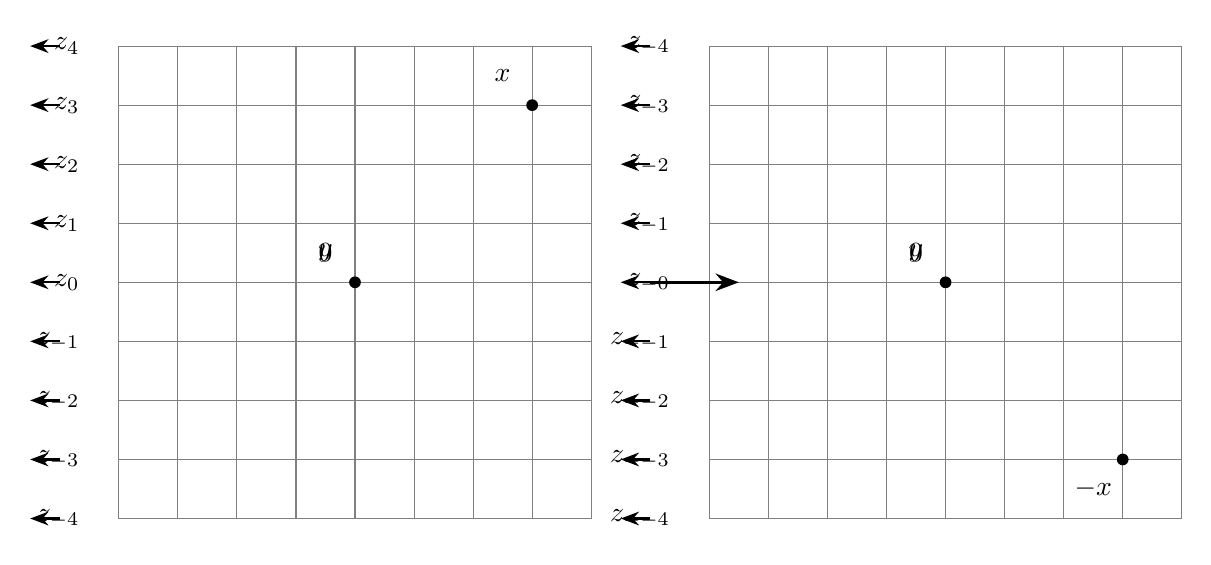
\begin{tikzpicture}[scale=0.75]

% Define some styles for consistency
\tikzset{
    gridline/.style={thin, gray},
    arrow/.style={->, >=Stealth, thick},
    label/.style={anchor=east, black},
    node/.style={circle, fill=black, inner sep=1.5pt},
}

% Left Grid
\foreach \i in {-4,...,4} {
    \draw[gridline] (\i, -4) -- (\i, 4);
    \draw[gridline] (-4, \i) -- (4, \i);
    \node[label] at (-4.5, \i) {$z_{\i}$};
}

% Arrows and Labels for Left Grid
\foreach \i in {-4,...,4} {
    \draw[arrow] (-5, \i) -- ++(-0.5, 0);
}
\node[node] at (3, 3) {};
\node[node] at (0, 0) {};
\node at (2.5, 3.5) {$x$};
\node at (-0.5, 0.5) {$y$};
\node at (-0.5, 0.5) {$0$};

% Right Grid
\begin{scope}[xshift=10cm]
    \foreach \i in {-4,...,4} {
        \draw[gridline] (\i, -4) -- (\i, 4);
        \draw[gridline] (-4, \i) -- (4, \i);
        \node[label] at (-4.5, \i) {$z_{-\i}$};
    }

    % Arrows and Labels for Right Grid
    \foreach \i in {-4,...,4} {
        \draw[arrow] (-5, \i) -- ++(-0.5, 0);
    }
    \node[node] at (0, 0) {};
    \node[node] at (3, -3) {};
    \node at (-0.5, 0.5) {$0$};
    \node at (2.5, -3.5) {$-x$};
    \node at (-0.5, 0.5) {$y$};
\end{scope}

% Arrow Between Grids
\draw[arrow, very thick] (5, 0) -- ++(1.5, 0);

\end{tikzpicture}

\end{document}